\chapter{Finding 1: Corrupted Early Timing Advance}
\label{ch:m1}

\section{Threat Model and Capabilities}
\label{sec:threat}

The adversary requires only two capabilities established in published literature and feasible with
commodity hardware:
\begin{enumerate}\itemsep2pt
  \item \textbf{Passive Downlink Sniffing:} The adversary decodes unencrypted physical-layer control
        information (DCI on PDCCH) using a passive receiver (e.g., 5GSniffer~\cite{ludant2023sniffing}).
        This reveals when an early PRACH transmission has been scheduled for a target candidate cell.
  \item \textbf{Radio-Frequency (RF) Relay:} The adversary captures the UE's PRACH preamble over the air
        and forwards it toward the candidate cell with an intentional propagation delay $\Delta$, without
        altering the preamble payload.
\end{enumerate}
The adversary possesses no cryptographic keys, cannot compromise gNB/UE internals, and does not forge
RRC messages. Crucially, this attack requires no forged MAC CEs, allowing it to survive future MAC CE
integrity protection.

\section{The Early Timing Advance Vulnerability}
\label{sec:m1attack}

Three architectural characteristics in 3GPP specifications enable the attack:

\subsection{Absence of Device-to-Preamble Binding}
When the serving gNB orders early \TA{} acquisition, the candidate cell is informed of three parameters:
the target cell ID, the assigned preamble index, and the PRACH occasion. It receives no cryptographic
token, UE identity (C-RNTI), or authentication tag. The candidate gNB correlates all incoming energy
in that occasion against the preamble sequence and extracts the timing offset corresponding to the
highest correlation peak. If an adversary forwards a delayed copy of the preamble with sufficient
power, the candidate cell accepts the delayed peak as legitimate, recording an inflated round-trip time.

\begin{figure}[htbp]
  \centering
  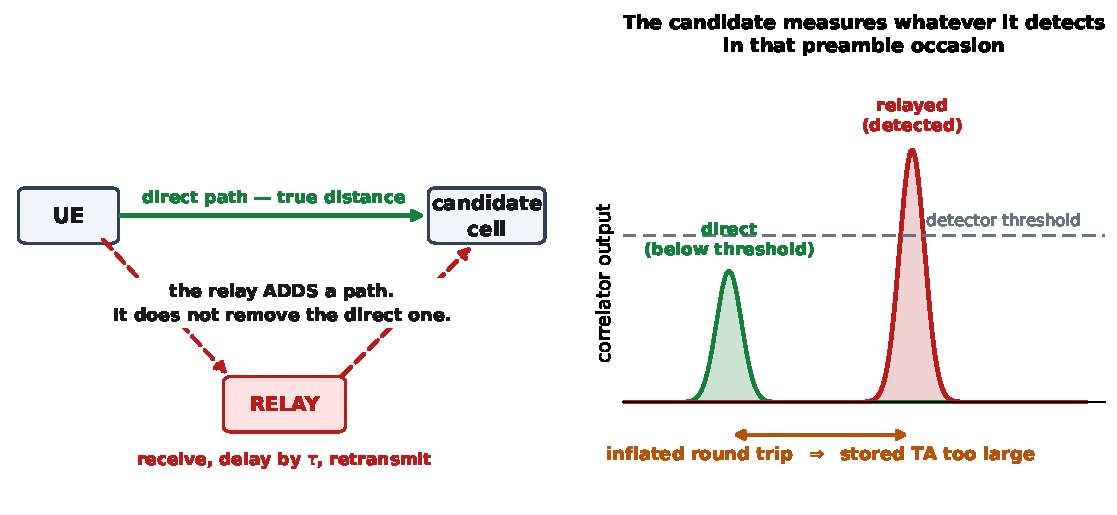
\includegraphics[width=\textwidth]{figures/atk05_relay.pdf}
  \caption{RF relay geometry. The candidate gNB correlates both the direct UE preamble and the
  delayed relayed copy. The attack succeeds when the relayed correlation peak exceeds the direct path.}
  \label{fig:relay}
\end{figure}

\subsection{Scope: Network-Supplied Candidate \TA{}}
\label{sec:m1scope}
Under TS~38.321 clause~5.2 and TS~38.213 clause~21~\cite{3gpp38213,3gpp38321}, an LTM switch obtains
its candidate \TA{} via one of two paths:
\begin{itemize}\itemsep2pt
  \item \textbf{Network-Supplied \TA{}:} The 12-bit Timing Advance Command in the LTM Cell Switch Command
        MAC CE contains an explicit integer value ($\ne \texttt{0xFFF}$). This value is populated by
        early acquisition.
  \item \textbf{UE-Measured \TA{}:} The Timing Advance Command is set to \texttt{0xFFF}, instructing the
        UE to reuse serving cell timing (applicable only to co-sited, synchronized candidates).
\end{itemize}
Our attack specifically targets the network-supplied path, which is universally required for inter-site
mobility across non-colocated base stations.

\subsection{Unbounded Network-Side Retention}
\label{sec:m1retention}
Once measured, the candidate \TA{} is transmitted across internal F1-C interfaces via the F1AP
\texttt{DU-CU TA INFORMATION TRANSFER} procedure~\cite{3gpp38473}. Remarkably, the F1AP Information
Element carries the cell ID, \TA{} value, preamble index, and RA-RNTI, but contains no timestamp,
sequence counter, or validity lifetime timer. TS~38.300 clause~9.2.3.5.2 states plainly that the UE does
not maintain a TA timer for the candidate cell, and that validity instead relies entirely on network
implementation~\cite{3gpp38300}. Because 3GPP specifies no retention limit, the serving cell may cache
this corrupted \TA{} indefinitely.
The adversary can execute the relay attack during an early preparation phase and depart; the damage is
only triggered when the network later issues the switch command.

\section{Theoretical Decodability Limit and Numerology Invariance}
\label{sec:m1boundary}

In 5G NR, the normal cyclic prefix duration is $L_{\mathrm{CP}} = 144 \cdot 64 \cdot T_c / 2^{\mu}$.
Dividing this by the basic timing advance unit $T_{\mathrm{unit}}$ from \cref{eq:taunit} yields:
\begin{equation}
  \frac{L_{\mathrm{CP}}}{T_{\mathrm{unit}}}
  = \frac{144 \cdot 64 \cdot T_c / 2^{\mu}}{16 \cdot 64 \cdot T_c / 2^{\mu}}
  = \frac{144}{16} = 9 \quad \text{\TA{} units, at all numerologies } \mu.
  \label{eq:cp9}
\end{equation}
The numerology scaling factor $2^{-\mu}$ cancels identically. Consequently, the theoretical cyclic prefix
guard interval spans exactly $9\,T_{\mathrm{unit}}$ regardless of subcarrier spacing ($\mu \in \{0, 1, 2, 3\}$).
In real propagation channels, multipath delay spread consumes a fraction of this guard interval; the exact
empirical failure cliff under realistic channel models is evaluated experimentally in \cref{ch:results}.

\section{Relay Feasibility and Link-Budget Geometry}
\label{sec:m1delay}

For the relay's forwarded signal to capture the candidate gNB's PRACH correlator, its received power at
the gNB must exceed the direct UE path by a threshold $\Delta_{\mathrm{th}}$:
\begin{equation}
  \underbrace{(P_{\mathrm{relay}} - P_{\mathrm{UE}})}_{\text{Power Advantage}}
  - \underbrace{\bigl(\mathrm{PL}(r) - \mathrm{PL}(d)\bigr)}_{\text{Path-Loss Disadvantage}}
  \;\ge\; \Delta_{\mathrm{th}} ,
  \label{eq:linkbudget}
\end{equation}
where $d$ is the candidate-to-UE distance, $r$ is the candidate-to-relay distance, and $\mathrm{PL}(\cdot)$
is path loss in dB modeled via 3GPP TR~38.901~\cite{3gpp38901}. Throughout this section, $\Delta_{\mathrm{th}}$
is not an assumed constant: it is the empirical 90\% capture threshold established experimentally via
srsRAN simulation in \cref{sec:r1capture} ($+9.9$\,dB under flat fading, $+5.3$\,dB under urban multipath),
substituted here to project relay feasibility over distance and power.

\begin{table}[htbp]
  \centering
  \caption{Maximum allowable candidate-to-relay distance $r$ achieving 90\% capture threshold
  ($\Delta_{\mathrm{th}} = +9.9$\,dB for flat fading; $+5.3$\,dB for urban multipath), 3.5\,GHz UMa NLOS,
  at two representative macro-cell victim distances. The ratio $r/d$ is distance-invariant (confirmed
  across 200\,m--2\,km in \cref{fig:capture}, right panel), so only $d=500$\,m and $d=1000$\,m are shown
  here; the same ratios apply at any $d$.
  Analytic projection from the TR~38.901 path-loss model (\cref{eq:linkbudget}), not a Monte Carlo
  measurement.}
  \label{tab:link}
  \small
  \begin{tabular}{@{}lrr@{}}
    \toprule
    Relay Power Advantage & $d=500$\,m & $d=1000$\,m \\
    \midrule
    \multicolumn{3}{@{}l}{\emph{Flat Rayleigh Fading ($\Delta_{\mathrm{th}} = +9.9$\,dB)}} \\
    $0$\,dB (23\,dBm)   & 275\,m  & 555\,m  \\
    $+10$\,dB (33\,dBm) & 500\,m  & 1005\,m \\
    $+20$\,dB (43\,dBm) & 905\,m  & 1810\,m \\
    \addlinespace
    \multicolumn{3}{@{}l}{\emph{Urban Multipath Profile ($\Delta_{\mathrm{th}} = +5.3$\,dB)}} \\
    $0$\,dB (23\,dBm)   & 365\,m  & 730\,m  \\
    $+10$\,dB (33\,dBm) & 655\,m  & 1315\,m \\
    $+20$\,dB (43\,dBm) & 1185\,m & 2375\,m \\
    \bottomrule
  \end{tabular}
\end{table}

As shown in \cref{tab:link}, a relay radiating 33\,dBm (a modest 10\,dB advantage over a standard 23\,dBm
handset) achieves capture from any location where $r \le d$. Under urban multipath, the required margin
drops to 5.3\,dB, expanding the operational zone to $r \le 1.3\,d$. Thus, the attacker faces no delicate
positioning constraints.

Furthermore, an induced delay of seven units at $\mu=1$ corresponds to $7 \times 260.4\,\text{ns} = 1.82\,\mu\text{s}$,
equivalent to an excess propagation path of $547$\,m. An adversary can introduce this delay entirely
geometrically by positioning itself off the direct line-of-sight path between the UE and the candidate cell.

\section{Analysis of Network-Controlled Repeaters (NCR)}
\label{sec:m1ncr}

3GPP Release 18 standardized Network-Controlled Repeaters (NCR) as low-cost coverage
extenders~\cite{3gpp38867,carvalho2024ncr}.
Because repeaters introduce group delay, it is essential to determine whether deployed repeaters already
induce this failure accidentally, or whether an active adversary is required.

\begin{table}[htbp]
  \centering
  \caption{Forwarding delay of relay/repeater technologies at $\mu=1$ ($260.4$\,ns per \TA{} unit). The
  SDR figure is the receive-path latency reported directly in~\cite{usrplatency} (not a derived or
  halved round-trip estimate).}
  \label{tab:hardware}
  \small
  \begin{tabularx}{\textwidth}{@{}l r r X@{}}
    \toprule
    Hardware Type & Latency & \TA{} Units & Impact on Attack Feasibility \\
    \midrule
    Host-controlled SDR~\cite{usrplatency} & 57.6--126\,$\mu$s & 221--484 & Exceeds PRACH search window \\
    FPGA loopback relay~\cite{nifpgaloopback} & 550\,ns & 2.1 & Requires buffer to reach 7 units \\
    Commercial digital repeater~\cite{ti2018repeater} & 2--6\,$\mu$s & 7.7--23.0 & Readily exceeds 7 units \\
    3GPP Release-18 NCR~\cite{3gpp38867,carvalho2024ncr} & tens of ns & $\sim$0.1 & Negligible delay; fails harmlessly \\
    \bottomrule
  \end{tabularx}
\end{table}

As shown in \cref{tab:hardware}, standardized 3GPP NCRs operate with analog RF filtering latencies under
50\,ns (consuming $<0.2\,T_{\mathrm{unit}}$), which is harmless. Furthermore, in legacy networks, repeater
propagation delays are \textbf{common-mode}: because the same physical path is used during both RACH
estimation and subsequent data transmission, static delays cancel out naturally.

Early acquisition breaks this common-mode cancellation. The \TA{} is measured across one path (e.g.,
through an adversary's relay), stored indefinitely, and subsequently applied across a different path
during RACH-less handover. What an adversary supplies is not absolute delay, but \textbf{differential
delay} that is frozen into network state.
